\begin{addmargin}[6cm]{} % Adiciona margim de recuo no texto

É possível observar que, a CDA supracitada foi emitida com posição de 06/08/2021, considerando que, nesta data, o valor de juros de mora da multa punitiva remonta em R\$ 388.009,45 sobre o valor principal da multa de R\$ 484.830,00, ou seja, depreende-se que o percentual de juros aplicado é de 80,04\%.
    \begin{itemize}
        \item \textbf{Qual foi a Taxa SELIC acumulada neste mesmo período?}

    \textbf{Resposta:} Considerando que se trata de novo posicionamento temporal de comparação, a \textbf{Perícia} perseguiu a Taxa SELIC acumulada considerando os parâmetros de termo inicial (outubro de 2012) e data do posicionamento da CDA de fl. 349 (agosto de 2021), na própria fonte de cálculo dos débitos tributários administrados pela União (sítio da Receita Federal do Brasil ), constatando que, a Taxa SELIC acumulada perfaz \textbf{74,79\%} para o mesmo período, vejamos:

\begin{figure}[!h]
    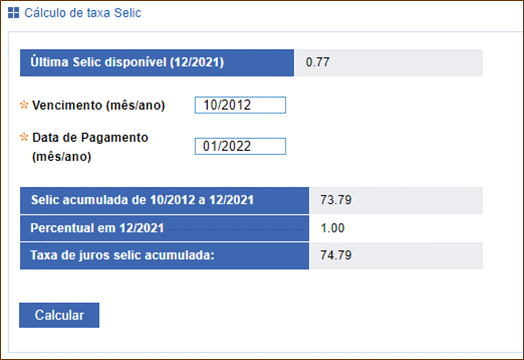
\includegraphics{Imagens/Taxa SELIC acumulada extraída do SICALC (Programa de Atualização Débitos da RFB).png}
    \caption{Taxa SELIC acumulada extraída do SICALC (Programa de Atualização Débitos da RFB)}
    \label{fig:my_label}
\end{figure}

%\newgeometry{left = 8cm} %muda a margem esquerda para 5cm
 \item \textbf{Podemos afirmar que os percentuais aplicados pela FESP para cálculo dos juros de mora da multa punitiva são superiores à Taxa SELIC?}
\textbf{Resposta:} Positiva é a resposta. Em virtude da aplicação da taxa de \textbf{80,04\%} em detrimento dos limites da Taxa SELIC acumulada, a qual resultou em \textbf{74,79\%} para o mesmo período.

\item \textbf{Podemos afirmar que ao aplicarmos a Taxa SELIC para cálculo dos juros de mora da multa punitiva o valor final efetivamente devido pela Autora a título de juros de mora da multa punitiva será reduzido?}

\textbf{Resposta:} Positiva é a resposta, aplicando a taxa de \textbf{74,79\%} identificada no próprio programa que acumula a Taxa SELIC e que remunera os débitos federais (tese da \textbf{Requerente}), o resultado dos juros de mora da multa punitiva perfaz o montante de \textbf{R\$ 350.252,70} já considerando que o percentual de \textbf{74,79\%} seja aplicado sobre a multa punitiva recalculada no valor de \textbf{R\$ 468.314,88}, sendo inferior ao montante calculado originalmente na CDA de fl. 349 dos autos, em referência ao quanto perquirido no quesito.
%\newgeometry{left = 3cm}
\end{itemize}
\end{addmargin}
